\subsection{DirectX.NET}

\subsubsection{Czym jest DirectX.NET}

Pojawienie się w 1995 pierwszej wersji DirectX, przeznaczonej dla nowo zaprojektowanego systemu 
operacyjnego Windows 95, oznaczało ostateczne otwarcie się świata Windows na zaawansowane 
aplikacje multimedialne. Celem projektantów DirectX było stworzenie jednolitego interfejsu 
programowania, który pozwoliłby programistom tworzyć kod dający się uruchomić na dowolnie 
skonfigurowanym PC-cie. 

Niemal od samego początku DirectX był przez programistów mocno krytykowany. 
Krytyka była szczególnie zjadliwa, gdy porównywano DirectX do OpenGL - mimo dość dużych różnic 
technologicznych, programistom trudno było wytłumaczyć dlaczego kod w DirectX musi być tak brzydki i 
zagmatwany w porównaniu z analogicznym kodem w OpenGL. 	

Pojawienie się platformy .NET i języka C\# dawało nadzieję na zmianę tej sytuacji. Jednak 
okazało się, że programiści owszem, mogą korzystać z DirectX, ale wymaga to warstwy pośredniej 
między DirectX 8 zbudowanym w modelu COM, a kodem zarządzanym. Dopiero pojawienie się DirectX 9 
oznacza prawdziwy przełom. Zgodnie z obietnicami, Microsoft dołączył do najnowszej wersji 
DirectX 9.0 zestaw bibliotek, umożliwiających korzystanie z DirectX bezpośrednio z poziomu kodu 
zarządzanego. Biblioteki te nazwano DirectX.NET. 

Możliwość bezpośredniego operowania obiektami DirectX z poziomu kodu zarządzanego ma mnóstwo zalet, m.in.:
\begin{itemize}
\item kod w pełni zarządzany jest znacznie prostszy, interfejs DirectX.NET jest bardzo intuicyjny
\item kod zarządzany oznacza brak zmartwień związanych z obsługą błędów i zarządzaniem pamięcią
\item brak pośredniej warstwy między COM a kodem zarządzanym oznacza większą szybkość kodu DirectX
\end{itemize}

DirectX.NET jest nareszcie porządnym interfejsem zorientowanym obiektowo. Do tej pory interfejs 
DirectX był przedziwną mieszaniną funkcji globalnych, makr i klas, a wszystko to podlane było ciężkostrawnym 
sosem modelu COM.

Dość już magicznych funkcji do operacji na obiektach. Teraz zamiast:

\begin{scriptsize}
\begin{verbatim}
D3DXMATRIX turnLeft;
D3DXMatrixRotationY( &turnLeft, -10.0 );
\end{verbatim}
\end{scriptsize}

napiszemy:

\begin{scriptsize}
\begin{verbatim}
Matrix turnLeft = Matrix.RotationY( -10.0f );
\end{verbatim}
\end{scriptsize}

Dość już magicznych stałych, teraz zamiast:

\begin{scriptsize}
\begin{verbatim}
_device->SetRenderState(D3DRS_LIGHTING, true);
\end{verbatim}
\end{scriptsize}

napiszemy:

\begin{scriptsize}
\begin{verbatim}
_device.RenderState.Lighting = true;
\end{verbatim}
\end{scriptsize}

Dość ciągłych {\tt HRESULT}ów i makr {\tt SUCCEEDED/FAILED}. Teraz błędy zgłaszane są za pomocą wyjątków. 
Dość tysięcy typów danych, jak choćby {\tt D3DCOLOR} - biblioteki DirectX.NET są zintegrowane z biblioteką 
standardową .NET, a to oznacza że teraz użyjmy po prostu {\em System.Drawing.Color}. 

A jak jest z wydajnością? Zaskakująco dobrze - zarządzany DirectX jest niewiele lub prawie wcale 
wolniejszy od niezarządzanego. Decydujące znaczenie dla prędkości działania kodu ma najczęściej i tak 
wydajność akceleratora, zaś prędkość wykonywania się samego kodu jest porównywalna. 

\subsubsection{Struktura DirectX.NET}

Zarządzane biblioteki DirectX są wspólne dla wszystkich języków platformy .NET. 
Należy pamiętać o tym, że tylko w C++ można tworzyć kod DirectX "po staremu", czyli nie korzystając 
z obiektowych bibliotek zarządzanych.

DirectX.NET składa się z następujących komponentów:
\begin{description}
\item [Direct3D] - interfejs do programowania efektów 3D
\item [DirectDraw] - niskopoziomowy dostęp do grafiki 2D
\item [DirectInput] - obsługa różnych urządzeń wejściowych, łącznie z pełnym wsparciem technologii force-feedback.
\item [DirectPlay] - wsparcie dla gier sieciowych gier wieloosobowych 
\item [DirectSound] - tworzenie i przechwytywanie dźwięki
\item [Audio Video Playback] - kontrola nad odtwarzaniem zasobów audio i video
\end{description}

\subsubsection{Instalacja DirectX.NET}

Biblioteki DirectX.NET instalowane są automatycznie podczas instalacji DirectX 9. 
Ich obecność można zbadać zaglądając do katalogu Microsoft.NET w katalogu systemowym Windows. 
Oprócz katalogu Framework, gdzie domyślnie instaluje się .NET Framework, powinien być tam również 
katalog Managed DirectX. Programiści powinni pamiętać o wybraniu odpowiedniej wersji DirectX 9: 
oprócz wersji standardowej, w DirectX 9 SDK znajduje się specjalna wersja umożliwiająca również 
śledzenie kodu DirectX z poziomu środowiska (po zainstalowaniu SDK obie wersje znajdują się 
odpowiednio w {\em ./DX9SDK/SDKDev/Retail} lub {\em ./DX9SDK/SDKDev/Debug)}.

Natychmiast po zainstalowaniu DirectX9 SDK można zajrzeć do katalogu {\em ./Samples}, 
gdzie znajdują się przykładowe programy w C++, C\# i VB.NET. Spora część programów pojawia się we 
wszystkich tych językach, można więc porównać nie tylko przejrzystość kodu, ale i prędkość działania. 
Przykładów jest dużo i są naprawdę interesujące.

\begin{figure}
\begin{center}
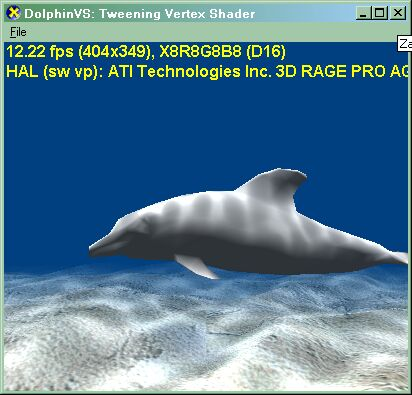
\includegraphics[width=0.75\textwidth]{./pic/dx0}
\caption{Jeden z przykładowych programów z DirectX 9 SDK}
\end{center}
\end{figure}

Programy DirectX.NET mogą być kompilowane zarówno z poziomu środowiska Visual Studio .NET, 
bezpośrednio z linii poleceń ale także z poziomu na przykład Sharp Developa. 
Dla celów kompilacji z linii poleceń przygotujmy prosty skrypt (nazwijmy go {\tt compile.bat}):

\begin{scriptsize}
\begin{verbatim}
csc.exe "/lib:C:\WINNT\Microsoft.NET\Managed DirectX\v4.09.00.0900" 
/r:Microsoft.DirectX.dll %1
\end{verbatim}
\end{scriptsize}

Skrypt ten będziemy wołać z parametrem zawierającym nazwę kompilowanego programu. 
Jeśli kompilowany program będzie wymagał referencji do większej ilości bibliotek, 
wystarczy dodać je jako kolejne parametry.

\subsubsection{Pierwszy program w DirectX.NET}

Pierwszy i najprostszy programem jaki napiszemy będzie tworzył powierzchnię DirectDraw i 
kopiował jej zawartość do okna. Tak naprawdę będzie nam potrzebna jedynie instancja 
obiektu urządzenia DirectDraw oraz obiektu opisującego powierzchnię DirectDraw.

\begin{scriptsize}
\begin{verbatim}
private Device  draw      = null; 
private Surface primary   = null;
\end{verbatim}
\end{scriptsize}

Oba obiekty są tworzone i kojarzone - urządzenie z oknem, a powierzchnia z urządzeniem:

\begin{scriptsize}
\begin{verbatim}
draw = new Device(); 
draw.SetCooperativeLevel(this, CooperativeLevelFlags.Normal);
	. . .
SurfaceDescription description = new SurfaceDescription(); 
description.SurfaceCaps.PrimarySurface = true; 
primary = new Surface(description, draw);
\end{verbatim}
\end{scriptsize}

Ponieważ powierzchnia DirectDraw jest obiektem, wszelkie operacje takie jak rysowanie, 
blokowanie czy zamiana stron są po prostu metodami odpowiedniego obiektu. 
Prosty kształt narysujemy więc za pomocą metody:

\begin{scriptsize}
\begin{verbatim}
primary.DrawCircle( .... );
\end{verbatim}
\end{scriptsize}

a tekst za pomocą metody:

\begin{scriptsize}
\begin{verbatim}
primary.DrawText( ... );	
\end{verbatim}
\end{scriptsize}

Interfejs obiektowy sprawdza się zwłaszcza w przypadku środowisk z autouzupełnianiem kodu - 
tam programista nie musi nawet zaglądać do dokumentacji biblioteki, ponieważ wszystkie metody 
obiektu pojawią się natychmiast po wpisaniu kropki po nazwie obiektu.

Poniższy przykład można bez trudu rozbudować o prostą animację, dodać podwójne buforowanie oraz 
wyświetlanie obrazu na pełnym ekranie. Proponuję potraktować to jako ćwiczenie, zerkając 
w razie potrzeby do przykładów z SDK. 

\begin{scriptsize}
\begin{verbatim}
/* Wiktor Zychla, 2003 */
using System;
using System.Drawing;
using System.ComponentModel;
using System.Windows.Forms;
using Microsoft.DirectX;
using Microsoft.DirectX.DirectDraw;

namespace DirectXTutorial
{
    public class DirectDrawForm : System.Windows.Forms.Form
    {        
        private Device  draw      = null; 
        private Surface primary   = null; 
        private Clipper clip      = null; 

        static void Main() 
        {
          Application.Run(new DirectDrawForm());
        }

        public DirectDrawForm()
        {
           this.ClientSize = new System.Drawing.Size(292, 266);
           this.Name = "DirectDraw w oknie";
           this.Text = "DirectDraw w oknie";
           this.Resize      += new System.EventHandler(this.DDForm_SizeChanged);
           this.SizeChanged += new System.EventHandler(this.DDForm_SizeChanged);
           this.Paint       += 
	     new System.Windows.Forms.PaintEventHandler(this.DDForm_Paint);

           draw = new Device(); 
           draw.SetCooperativeLevel(this, CooperativeLevelFlags.Normal); 
           CreateSurfaces(); 
        }

        private void DDForm_Paint(object sender, System.Windows.Forms.PaintEventArgs e)
        {
           Draw();
        }
        
        private void DDForm_SizeChanged(object sender, System.EventArgs e)
        {
           Draw();
        }
        
        private void Draw()
        {
           if ( primary == null ) return;           
           if ( WindowState == FormWindowState.Minimized ) return;
            			
           Point p = this.PointToScreen( new Point( 0, 0 ) );
           primary.ColorFill( Color.Blue );
           primary.ForeColor = Color.White;
           primary.DrawText( p.X, p.Y, "Pierwszy program w DirectX.NET", false );
        }
                                
        private void CreateSurfaces()
        {
            SurfaceDescription description = new SurfaceDescription(); 

            description.SurfaceCaps.PrimarySurface = true; 
            primary     = new Surface(description, draw); 
            clip        = new Clipper(draw); 
            clip.Window = this; 
            primary.Clipper = clip; 
        }
    }
}
\end{verbatim}
\end{scriptsize}

\subsubsection{Direct3D}

\begin{figure}
\begin{center}
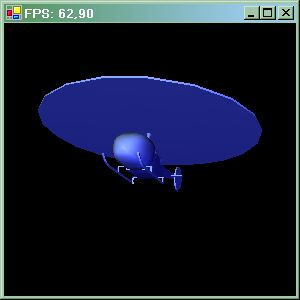
\includegraphics[width=0.50\textwidth]{./pic/dx1}
\caption{Trójwymiarowy świat Direct3D}
\end{center}
\end{figure}

Direct3D jest najciekawszą częścią DirectX.NET. W każdej kolejnej wersji DirectX programiści 
dostają do rąk coraz potężniejsze narzędzia do tworzenia grafiki 3D. W wersji 9 możliwości są 
przeogromne: od tworzenia prostych obiektów, modelowania światła, tekstur, przez manipulację 
siatkami obiektów ({\em vertex shading}) aż do zaawansowanego nakładania tekstur ({\em pixel shading}).  

Aby przekonać się jak sprawuje się obiektowy interfejs Direct3D, napiszemy prosty przykład. 
Z pliku załadujemy opis siatki obiektu 3d ({\em mesh}), dodamy 2 światła, kamerę i na koniec ożywimy 
całość dodając jakiś ruch.

\begin{scriptsize}
\begin{verbatim}
/* Wiktor Zychla, 2003 */
using System;
using System.Drawing;
using System.Windows.Forms;
using Microsoft.DirectX;
using Microsoft.DirectX.Direct3D;

namespace DirectXTutorial
{
  public class DirectXForm : Form 
  {
    Device   device;
    Mesh     mesh;
    int      meshParts = 0;
    Material material;
    float    rotationAngle = 0;
    PresentParameters pp;

    public DirectXForm() 
    {
      this.Size = new Size(300, 300);
      this.Text = "DirectX.NET";
    }

    bool InitializeGraphics() 
    {
      try
      {
        pp = new PresentParameters();
        pp.Windowed = true;
        pp.SwapEffect = SwapEffect.Discard;
        pp.EnableAutoDepthStencil = true;
        pp.AutoDepthStencilFormat = DepthFormat.D16;

        device = new Device(0, DeviceType.Hardware, this, 
	                    CreateFlags.SoftwareVertexProcessing, pp);
        device.DeviceReset += new EventHandler(OnDeviceReset);

        InitializeD3DObjects();

        return true;
      }
      catch (DirectXException)
      {
        return false;
      }
    }

    void InitializeD3DObjects() 
    {
      CreateMesh();
      CreateMaterials();
      CreateLights();
      InitializeView();
    }

    void OnDeviceReset(object o, EventArgs e) 
    {
      InitializeD3DObjects();
    }

    protected override void OnKeyPress(System.Windows.Forms.KeyPressEventArgs e)
    {
      if ((int)(byte)e.KeyChar == (int)Keys.Escape)
        this.Close(); // zakończ 
    }

    void CreateMesh() 
    {
      //mesh = Mesh.Teapot( device );
      //meshParts = 1;

      ExtendedMaterial[] m = null;

      mesh = Mesh.FromFile( "heli.x", 0, device, out m );
      meshParts = m.Length;
    }

    void CreateMaterials() 
    {
      material = new Material();
      material.Ambient = Color.FromArgb( 0, 80, 80, 80);
      material.Diffuse = Color.FromArgb(0, 200, 200, 200);
      material.Specular = Color.FromArgb(0, 255, 255, 255);
      material.SpecularSharpness = 128.0f;
    }

    void CreateLights() 
    {
      Light light0 = device.Lights[0];
      Light light1 = device.Lights[1];

      light0.Type = LightType.Directional;
      light0.Direction = new Vector3(-1, 1, 5);
      light0.Diffuse = Color.Blue;
      light0.Enabled = true;
      light0.Commit();

      light1.Type = LightType.Spot;
      light1.Position  = new Vector3(-10, 10, -50);
      light1.Direction = new Vector3(10, -10, 50);
      light1.InnerConeAngle = 0.5f;
      light1.OuterConeAngle = 1.0f;
      light1.Diffuse        = Color.LightBlue;
      light1.Specular       = Color.White;
      light1.Range          = 1000.0f;
      light1.Falloff        = 1.0f;
      light1.Attenuation0   = 1.0f;
      light1.Enabled        = true;
      light1.Commit();

      device.RenderState.Lighting = true;
      device.RenderState.DitherEnable = false;
      device.RenderState.SpecularEnable = true;
      device.RenderState.Ambient = Color.FromArgb(0, 20, 20, 20);
    }

    void InitializeView() 
    {
      Vector3 eyePosition = new Vector3(0, 0, -20);
      Vector3 direction   = new Vector3(0, 0, 0);
      Vector3 upDirection = new Vector3(0, 1, 0);

      Matrix view = Matrix.LookAtLH(eyePosition, direction, upDirection );
      device.SetTransform(TransformType.View, view);

      float fieldOfView = (float)Math.PI/4;
      float aspectRatio = 1.0f;
      float nearPlane   = 1.0f;
      float farPlane    = 500.0f;

      Matrix projection = Matrix.PerspectiveFovLH(fieldOfView, 
                            aspectRatio, nearPlane, farPlane);
      device.SetTransform(TransformType.Projection, projection);
    }

    void AdvanceFrame() 
    {
      rotationAngle += 0.02f;
      rotationAngle %= Geometry.DegreeToRadian(360);

      Matrix rotateX = Matrix.RotationX(rotationAngle);
      Matrix rotateY = Matrix.RotationY(rotationAngle);
      Matrix world = Matrix.Multiply(rotateX, rotateY);
      device.SetTransform( TransformType.World, world );
    }

    void Render() 
    {
      device.Clear(ClearFlags.Target | ClearFlags.ZBuffer, 
                   Color.Black.ToArgb(), 1.0f, 0);
      device.BeginScene();
      device.Material = material;

      for ( int i=0; i<meshParts; i++ )
        mesh.DrawSubset(i);

      device.EndScene();
      device.Present();
    }

    public static void Main() 
    {
      using ( DirectXForm dxForm = new DirectXForm() )
      {
        if (!dxForm.InitializeGraphics()) 
        {
          MessageBox.Show( "Błąd inicjowania Direct3D." );
          return;
        }
			
        dxForm.Show();

        DateTime start = DateTime.Now;
        int      frame = 0;
        while ( dxForm.Created )
        {
          frame++;
          dxForm.AdvanceFrame();
          dxForm.Render();

          dxForm.Text = String.Format( "FPS: {0:N}", 
	             frame/((TimeSpan)(DateTime.Now-start)).TotalSeconds );
          Application.DoEvents();
        }
      }
    }
  }
}
\end{verbatim}
\end{scriptsize}
 
Przyjrzyjmy się przykładowemu fragmentowi, który tworzy macierze widoku i perspektywy i po 
raz kolejny zwróćmy uwagę jak elegancko spisuje się tutaj model obiektowy DirectX.NET:

\begin{scriptsize}
\begin{verbatim}
Vector3 eyePosition = new Vector3(0, 0, -20);
Vector3 direction   = new Vector3(0, 0, 0);
Vector3 upDirection = new Vector3(0, 1, 0);
Matrix view = Matrix.LookAtLH(eyePosition, direction, upDirection );
device.SetTransform(TransformType.View, view);
float fieldOfView = (float)Math.PI/4;
float aspectRatio = 1.0f;
float nearPlane   = 1.0f;
float farPlane    = 500.0f;
Matrix projection = Matrix.PerspectiveFovLH(fieldOfView, aspectRatio, 
  nearPlane, farPlane);
device.SetTransform(TransformType.Projection, projection);
\end{verbatim}
\end{scriptsize}

Na uwagę zasługuje także nieco inna niż w typowej aplikacji okienkowej konstrukcja pętli głównej programu, 
dzięki której uzyskuje się maksymalną możliwą wydajność animacji. 

Otóż w zwykłej aplikacji okienkowej w C\# w funkcji Main pisze się najczęściej po prostu:

\begin{scriptsize}
\begin{verbatim}
Application.Run( new fMain() );
\end{verbatim}
\end{scriptsize}

Jednak przy takiej konstrukcji aby uzyskać jakikolwiek ruch musielibyśmy utworzyć zegar, 
ustawić go na jakiś kwant czasu i podczas obsługi zdarzenia zegara tworzyć kolejną ramkę animacji. 
Takie rozwiązanie ma dużą wadę: zakładamy bowiem że kwant czasu zaprogramowanego zegara odpowiada mniej 
więcej możliwości tworzenia płynnego obrazu przez maszynę. O wiele lepiej byłoby tworzyć obraz 
natychmiast po tym, kiedy skończy się tworzenie poprzedniej ramki. 

W pierwszej chwili wydaje się, że wymagałoby to zejścia aż na poziom pętli obsługi komunikatów, 
jednak nieoczekiwane, jest to możliwe w C\# na poziomie kodu obiektowego:

\label{netPetlaObslugiKomunikatow}

\begin{scriptsize}
\begin{verbatim}
using ( DirectXForm dxForm = new DirectXForm() )
{
  . . .			
  dxForm.Show();
  . . .
  while ( dxForm.Created )
  {
    dxForm.AdvanceFrame();
    dxForm.Render();

    Application.DoEvents();
  }
}
\end{verbatim}
\end{scriptsize}

Podobnie jak w przypadku DirectDraw, proponuję ten prosty przykład potraktować jako szablon do 
dalszych eksperymentów. 

